\documentclass[a4paper,11pt]{article}
\usepackage[utf8]{inputenc}
\usepackage{amsmath, amssymb}
\usepackage{graphicx}
\usepackage{listings}
\usepackage{xcolor}
\usepackage{geometry}
\geometry{margin=2.5cm}

\usepackage{hyperref}
\hypersetup{
    colorlinks,
    citecolor=black,
    filecolor=black,
    linkcolor=black,
    urlcolor=black
}

\usepackage{titling}
\renewcommand\maketitlehooka{\null\mbox{}\vfill}
\renewcommand\maketitlehookd{\vfill\null}

\title{\Huge{\textbf{Modèle de Cox-Ross-Rubinstein}}\\ \medskip
      \Huge{\textit{Compte rendu du TP - MAP552}}\vspace*{0.7cm}}
\author{\LARGE{Alexis VO}\vspace{1cm}\\ \medskip
      Université Paris-Saclay\\École polytechnique}
\date{\vspace{0.2cm}\today}

\lstset{
  language=Python,
  basicstyle=\ttfamily\footnotesize,
  keywordstyle=\color{blue},
  commentstyle=\color{gray},
  stringstyle=\color{red},
  showstringspaces=false,
  frame=single
}

\begin{document}

\maketitle
\newpage
\tableofcontents
\vspace{1cm}

\noindent \textit{Toutes les implémentations sont en Python, avec les librairies NumPy, Scipy et Matplotlib.}

\newpage

\section{Modèle binomial à $n$ périodes}

On considère un actif avec prix initial $S_0$, maturité $T$, drift $\mu$, volatilité $\sigma$, et $n$ périodes.

Le pas de temps est :
\(
h_n = \frac{T}{n}
\)

Les coefficients d'évolution sont définis par :
\[ u_n = e^{\mu h_n + \sigma \sqrt{h_n}}\]
\[ d_n = e^{\mu h_n - \sigma \sqrt{h_n}} \]

Les prix possibles à la date $j$ sont donnés par :
\[
\boxed{S_j^{(i)} = S_0 \cdot u^{j - i} d^i, \quad \text{pour } i = 0, 1, \dots, j \text{ et } S_0 > 0}
\]

\textbf{Implémentation :}
\begin{lstlisting}
def Sn(T, n, mu, sigma, j):
    h = T / n
    u = np.exp(mu * h + sigma * np.sqrt(h))
    d = np.exp(mu * h - sigma * np.sqrt(h))
    return np.array([S0 * u**(j - i) * d**i for i in range(j + 1)])
\end{lstlisting}

\section{Option européenne de type call}

Le gain à la maturité pour une option call de strike $K$ est :
\[
\boxed{\text{Payoff}(i) = \max(S_n^{(i)} - K, 0)}
\]

\textbf{Implémentation :}
\begin{lstlisting}
def Payoff(T, n, mu, sigma, K):
    prices = Sn(T, n, mu, sigma, n)
    return np.maximum(prices - K, 0)
\end{lstlisting}

\section{Évaluation backward : prix de l'option}
On utilise la \textit{probabilité risque-neutre} :
\( q = \frac{e^{r h} - d}{u - d}\)

\noindent La formule backward est :
\[
\boxed{V_j^{(i)} = e^{-r h} \left( q V_{j+1}^{(i)} + (1 - q) V_{j+1}^{(i+1)} \right)}
\]

Pour avoir l'intuition de cette formule, on peut la voir comme une moyenne pondérée des valeurs futures de l'option, actualisée au temps présent. On estime la valeur actuelle \(V_j^{(i)}\) comme la valeur espérée sous mesure risque-neutre des deux états possibles au pas suivant :
\begin{itemize}
    \item montée : \(V_{j+1}^{(i)}\) avec probabilité \(q\)
    \item descente : \(V_{j+1}^{(i+1)}\) avec probabilité \(1 - q\)
\end{itemize}
Puis on actualise à aujourd'hui avec le facteur \(e^{-r h}\).\\
\textbf{Remarque :} la probabilité risque neutre \(q\) est calculée pour s'assurer que le modèle respecte l'absence d'arbitrage.\newpage

\textbf{Implémentation :}
\begin{lstlisting}
def Calln(T, n, r, mu, sigma, K):
    h = T / n
    u = np.exp(mu * h + sigma * np.sqrt(h))
    d = np.exp(mu * h - sigma * np.sqrt(h))
    q = (np.exp(r * h) - d) / (u - d)
    V = Payoff(T, n, mu, sigma, K)
    for j in range(n - 1, -1, -1):
        V = np.exp(-r * h) * (q * V[:-1] + (1 - q) * V[1:])
    return V[0]
\end{lstlisting}

\section{Delta-hedging}

La couverture à la date $j$ est :
\[
\boxed{\Delta_j^{(i)} = \frac{V_{j+1}^{(i)} - V_{j+1}^{(i+1)}}{S_{j+1}^{(i)} - S_{j+1}^{(i+1)}}}
\]
où l'on a :
\begin{itemize} 
    \item \(V_{j+1}^{(i)}\) : valeur de l'option à la date $j+1$ dans l'état $i$
    \item \(V_{j+1}^{(i+1)}\) : valeur de l'option à la date $j+1$ dans l'état $i+1$
    \item \(S_{j+1}^{(i)}\) : prix de l'actif sous-jacent à la date $j+1$ dans l'état $i$
    \item \(S_{j+1}^{(i+1)}\) : prix de l'actif sous-jacent à la date $j+1$ dans l'état $i+1$
\end{itemize}
Cette formule nous donne la quantité d'actif à détenir pour couvrir l'option à la date $j$. Elle est calculée telle que \[\Delta = \frac{\text{variation de l'option}}{\text{variation de l'actif}}\]\\

\textbf{Implémentation :}
\begin{lstlisting}
def Deltan(T, n, r, mu, sigma, K, j):
    ...
    delta = (V_up - V_down) / (Sj1[:-1] - Sj1[1:])
    return delta
\end{lstlisting}

\section{Comparaison avec Black-Scholes}

Après avoir étudié la valorisation d’une option européenne dans le cadre discret du modèle binomial de Cox-Ross-Rubinstein, on va désormais s'intéresser à sa version continue : la formule de Black-Scholes. Cette dernière est la limite du modèle CRR quand le nombre de pas tend vers l’infini. Elle calcule directement le prix de l’option en fonction des paramètres du marché, sans avoir besoin de construire un arbre binomial comme dans le modèle CRR.\\

Formule de Black-Scholes :
\[
\boxed{C = S_0 \Phi(d_1) - K e^{-rT} \Phi(d_2)}
\]
avec :
\[
d_1 = \frac{\ln(S_0 / K) + (r + \frac{\sigma^2}{2})T}{\sigma \sqrt{T}}, \quad d_2 = d_1 - \sigma \sqrt{T}
\]

\textbf{Implémentation :}
\begin{lstlisting}
def Call(T, r, sigma, K):
    d1 = (np.log(S0 / K) + (r + sigma**2 / 2) * T) / (sigma * np.sqrt(T))
    d2 = d1 - sigma * np.sqrt(T)
    return S0 * norm.cdf(d1) - K * np.exp(-r * T) * norm.cdf(d2)
\end{lstlisting}

\section{Écart relatif et convergence}

\[
\boxed{\text{erreur}(n) = \frac{\text{Calln}(n)}{\text{Call}} - 1}
\]

\vspace{0.5cm}

\begin{center}
    \textbf{Graphe de l'erreur relative en fonction du nombre de périodes $n$}
    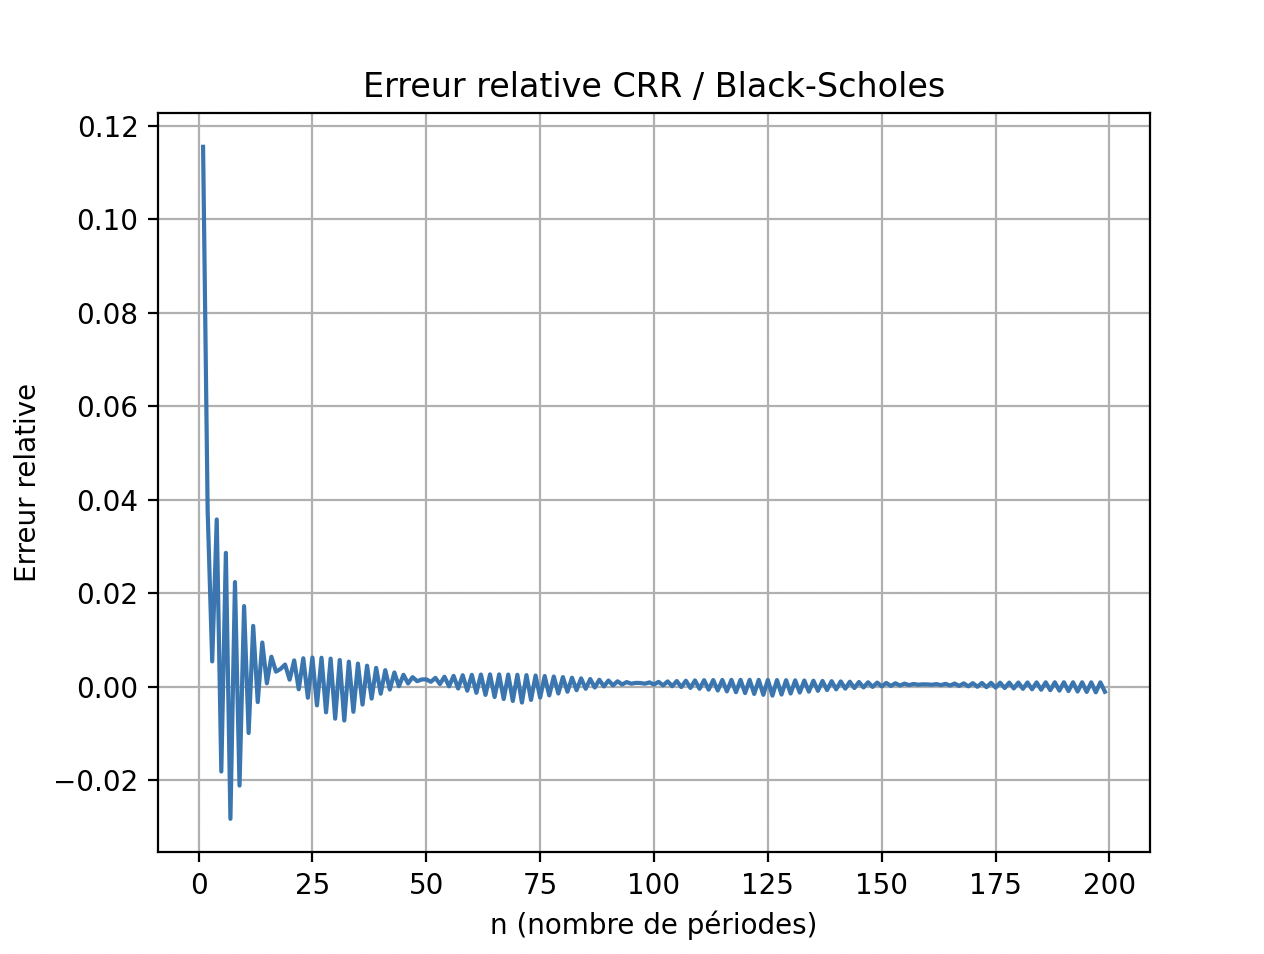
\includegraphics[width=0.8\textwidth]{error_plot.png}
\end{center}

\textbf{Interprétation :} on observe que l'erreur relative diminue lorsque le nombre de périodes $n$ augmente, ce qui confirme la convergence du modèle binomial vers la formule de Black-Scholes. Le graphe nous montre par ailleurs une décroissance rapide pour $n$ faible, puis un palier asymptotique vers 0 pour des valeurs plus élevées de $n$. La convergence est donc plus lente. On peut conclure que l'arbre binomial reste fiable pour des valeurs de $n$ relativement faibles.
\end{document}